\documentclass[hyperref,UTF8,11pt]{beamer}
\usepackage{ctex}
\usepackage[utf8]{inputenc}
\usepackage{fontspec}
\usepackage{comment}
%\setCJKfamilyfont{SimHei}
\usepackage{xeCJK}
%\renewcommand{\CJKfamilydefault}{\CJKsfdefault}
%\setmonofont{Consolas}
\setsansfont{Microsoft YaHei}
\setCJKmainfont{Microsoft YaHei}
%\setCJKmonofont{KaiTi}
%\setCJKsansfont{Microsoft YaHei}
\usefonttheme{professionalfonts}
\usepackage{hyperref}
\usepackage{graphicx}
\graphicspath{{image/}} % storage figure in a sub-folder
% \usepackage[parfill]{parskip} % Activate to begin paragraphs with an empty line rather than an indent
%\usepackage{epstopdf}
\usepackage{bm}
\usepackage{./style/nkcolor}
%\usepackage{hyperref}
\hypersetup{CJKbookmarks=true}
\usepackage{url}
\usepackage{amsmath}
\usepackage{amsthm}
\usepackage{calligra}

%\theoremstyle{definition}
%\newtheorem{theorem}{定理}
%\newtheorem{definition}{定义}
%\newtheorem{corollary}{推论}
%\newtheorem{example}{例}
\usepackage{booktabs} % for much better looking tables
%\usepackage{cite} % reference
\usepackage[backend=biber,style=numeric,sorting=none]{biblatex}
%\usepackage[backend=biber,style=apalike]{biblatex}
%\usepackage[backend=biber,style=authoryear]{biblatex}
% if style=apalike or authoryear, use \parencite instead of \cite
\addbibresource{./bibcite/nkthesis.bib}
\beamertemplatetextbibitems
\usepackage{array} % for better arrays (eg matrices) in maths
%\usepackage{paralist} % very flexible & customisable lists (eg. enumerate/itemize, etc.)
\usepackage{verbatim} % adds environment for commenting out blocks of text & for better verbatim
\usepackage{subfigure} % make it possible to include more than one captioned figure/table in a single float
% These packages are all incorporated in the memoir class to one degree or another...
%\usepackage{threeparttable}
\usepackage{cases} %equation set
\usepackage{multirow} %use table
\usepackage{enumerate}
\usepackage{algorithm}
\usepackage{algorithmic}
\usepackage{xcolor}
%\usepackage{capt-of}
\setcounter{tocdepth}{2}%只显示section,不显示subsection
\usepackage{listings}
\lstset{tabsize=4, keepspaces=true,
    xleftmargin=2em,xrightmargin=0em, aboveskip=1em,
    backgroundcolor=\color{gray!20},  % 定义背景颜色
    frame=none,                       % 表示不要边框
    extendedchars=false,              % 解决代码跨页时,章节标题,页眉等汉字不显示的问题
    numberstyle=\ttfamily,
    basicstyle=\ttfamily,
    keywordstyle=\color{blue}\bfseries,
    breakindent=10pt,
    identifierstyle=,                 % nothing happens
    commentstyle=\color{green}\small,  % 注释的设置
    morecomment=[l][\color{green}]{\#},
    numbers=left,stepnumber=1,numberstyle=\scriptsize,
    showstringspaces=false,
    showspaces=false,
    flexiblecolumns=true,
    breaklines=true, breakautoindent=true,breakindent=4em,
    escapeinside={/*@}{@*/},
}

\title[NN-ODE-PDE]{神经网络求ODE和PDE数值解}
\subtitle{NN for solve ODE and PDE}
\author[唐国鑫]{学生:唐国鑫\quad  \\ 导师:孙峪怀\quad \\\quad}
\institute[数学科学学院]{SICNU \quad 数学科学学院}
\date{\today} %Activate to display a given date or no date (if empty),
% otherwise the current date is printed

\begin{document}
%%%%%%%%%% 定理类环境的定义 %%%%%%%%%%
%% 必须在导入中文环境之后
\newcommand{\redstress}[1]{{\color{red}{#1}}}
%\renewcommand{\raggedright}{\leftskip=0pt \rightskip=0pt plus 0cm}
\renewcommand{\contentsname}{目录}     % 将Contents改为目录
\renewcommand{\abstractname}{摘要}     % 将Abstract改为摘要
\renewcommand{\refname}{参考文献}      % 将References改为参考文献
\renewcommand{\indexname}{索引}
\renewcommand{\figurename}{图}
\renewcommand{\tablename}{表}
\renewcommand{\appendixname}{附录}
%\renewcommand{\proofname}{证明}
%\renewcommand{\algorithm}{算法}
%----------------------------------------------------------------------
% Title frame
\begin{frame}
\maketitle
\end{frame}
%----------------------------------------------------------------------
\section{微分方程数值解的方法}
\begin{frame}{微分方程的一般数值解法}
\begin{block}{差分方法}
    \begin{itemize}
        \item Euler方法
        \item Taylor级数法
		\item Runge-Kutta方法
		\item 线性多步法
		\item Adams格式
		\item Gear格式
		\item ...
    \end{itemize}
\end{block}
\begin{block}{其它方法}
    \begin{itemize}
        \item 有限元法
    \end{itemize}
\end{block}
\end{frame}
%----------------------------------------------------------------------
%----------------------------------------------------------------------
\begin{frame}{微分方程的神经网络解法}
神经网络可以认为是一个强大的函数逼近器,通
过最小化损失函数来训练整个网络,下图
展示了CNN的拓扑结构\cite{2016Deep}:
    \begin{figure}
        \centering
        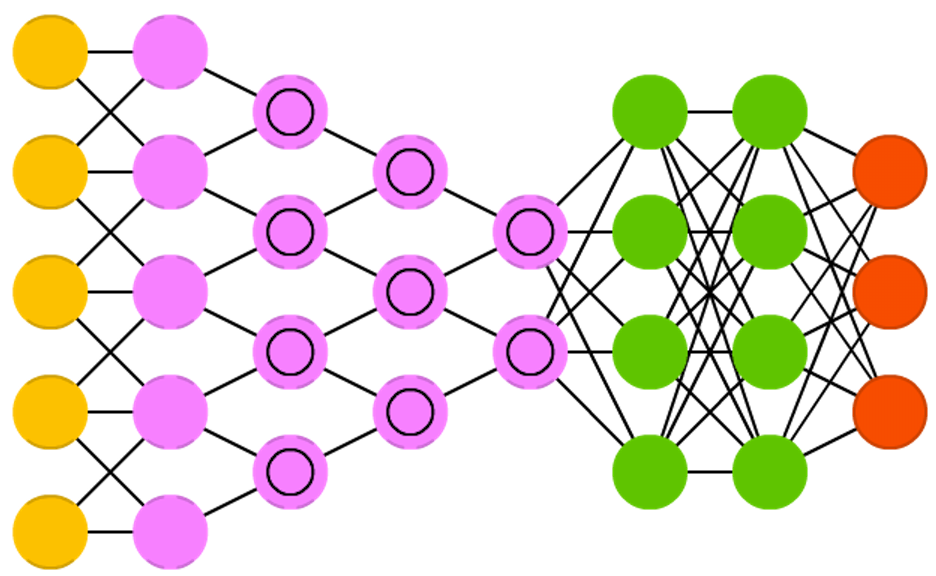
\includegraphics[width=0.7\textwidth]{./pic/cnn.png}
        \caption{卷积神经网络:CNN}\label{fig:CNN}
    \end{figure}

\end{frame}
%----------------------------------------------------------------------
\begin{frame}{微分方程的一般形式}
\begin{block}{连续形式}
	\begin{equation}
	G\left(\vec{x}, \Psi(\vec{x}), \nabla \Psi(\vec{x}), \nabla^{2} \Psi(\vec{x}), ...\right)=0, \vec{x} \in D
	\end{equation}
其中,$\vec{x}=\left(x_{1}, \ldots, x_{n}\right) \in R^{n}$,$D \subset R^{n}$.
\end{block}
\begin{block}{离散形式}
\begin{equation}
	G\left( {\overrightarrow {{x_i}} ,\Psi \left( {\overrightarrow {{x_i}} } \right),\nabla \Psi \left( {\overrightarrow {{x_i}} } \right),{\nabla ^2}\Psi \left( {\overrightarrow {{x_i}} } \right),...} \right) = 0,\forall \overrightarrow {{x_i}}  \in \hat D
\label{gde}
\end{equation}
\end{block}
\end{frame}
%----------------------------------------------------------------------
\begin{frame}{寻找损失函数}
如果$\Psi_{t}(\vec{x}, \vec{p})$是微分方程\eqref{gde}的一个试解,
那么求解微分方程数值解转化为下面的问题\cite{Lagaris1998Artificial}:
\begin{block}{Loss Function}
	\begin{equation}
	\min _{\vec{p}} \sum_{\overrightarrow{x_{i}} \in \hat{D}} G\left(\overrightarrow{x_{i}}, \Psi_{t}\left(\overrightarrow{x_{i}}, \vec{p}\right), \nabla \Psi\left(\overrightarrow{x_{i}}, \vec{p}\right), \nabla^{2} \Psi\left(\overrightarrow{x_{i}}, \vec{p}\right), ... \right)^{2}
	\end{equation}
\end{block}
其中,$\vec{p}$是神经网络的参数

\begin{block}{试解的构造}
	\begin{equation}
	\Psi_{t}(\vec{x})=A(\vec{x})+F(\vec{x}, N(\vec{x}, \vec{p}))
	\label{equ:try}
	\end{equation}
\end{block}
其中,$N(\vec{x}, \vec{p})$表示我们的神经网络$(NN)$,
$\vec{x}$为输入,$\vec{p}$为网络参数。$A$和$F$为满足边界的辅助函数。
\end{frame}
%----------------------------------------------------------------------

\begin{frame}{试解的构造方法}
\begin{block}{试解的构造形式}
	\begin{equation}
	\Psi_{t}(\vec{x})=A(\vec{x})+F(\vec{x}, N(\vec{x}, \vec{p}))
	\end{equation}
\end{block}
例如,对于下式常微分方程:
\begin{equation}
\frac{d^{2}}{d x^{2}} \Psi+\frac{1}{5} \frac{d}{d x} \Psi+\Psi=-\frac{1}{5} e^{-\frac{x}{5}} \cos x
\end{equation}
边界和初值为:$\Psi(0)=0$,$\frac{d}{d x} \Psi(0)=1$且$x \in[0,2]$。
我们构造的试解如下:
\begin{equation}
\Psi_{t}(x)=x+x^{2} N(x, \vec{p})
\end{equation}

解析解为:
\begin{equation}
\Psi(x)=e^{-\frac{x}{5}} \sin (x)
\end{equation}

\end{frame}


%----------------------------------------------------------------------
\section{NN的训练}
\begin{frame}{模型说明}
为了用神经网络求解微分方程,我们构造了如下的多层感知机(MLP)模型:
	\begin{columns}
        \begin{column}{0.4\textwidth}
            \begin{figure}
				\centering
				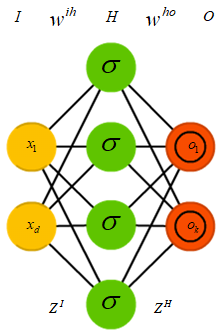
\includegraphics[width=0.6\textwidth]{./pic/nn.png}
				\caption{MLP模型}\label{fig:MLP}
			\end{figure}
        \end{column}
		
        \begin{column}{0.6\textwidth}
		\begin{block}{参数说明}
		\begin{enumerate}
			\item 输入/隐含/输出层:H/I/O
			\item 权重:$w^{ih}$/$w^{ho}$
			\item I层输入:$I=[x_1,x_2,...,x_d]$
			\item H层输入:$Z^I=Xw^{ih}$
			\item H层输出:$H=[h_1,h_2,...,h_h]$
			\item O层输入:$Z^H=Hw^{ho}$
			\item O层输出:$O=[o_1,o_2,...,o_k]$
			\item 激活函数:$\delta \left( X \right) = 1/\left( {1 + {e^{ - X}}} \right)$
		\end{enumerate}	
		\end{block}
        \end{column}
	\end{columns}
\end{frame}

%----------------------------------------------------------------------

\begin{frame}{训练方法}
神经网络的训练方法有很多,包括:
	\begin{block}{常见训练方法}
		\begin{enumerate}
			\item BP
			\item SGD
			\item ADAM
			\item BFGS
			\item LBFGS
			\item ...
		\end{enumerate}	
	\end{block}
	接下来我们主要推导BP算法,事实上,BP算法就是梯度下降法。
\end{frame}

%----------------------------------------------------------------------

\begin{frame}{BP算法}
    \begin{algorithm}[H]
        \caption{BP算法}\label{alg:em}
        \begin{algorithmic}[1]
            \REQUIRE $X$,$\eta$,$\varepsilon$,$Max	Iter$ and \eqref{equ:try}
            \ENSURE $w^{ih}$ and $w^{ho}$
            \REPEAT
            \STATE 计算$I=[x_1,x_2,...,x_d]$
			\STATE 计算H层输入:$Z^I=Xw^{ih}$
			\STATE 计算H层输出:$H=[h_1,h_2,...,h_h]$
			\STATE 计算O层输入:$Z^H=Hw^{ho}$
			\STATE 计算O层输出:$O=[o_1,o_2,...,o_k]$
			\STATE 更新O层与H层之间的梯度${w^{ho}} = {w^{ho}} + \eta \nabla {w^{ho}}$
			\STATE 更新H层与I层之间的梯度${w^{ih}} = {w^{ih}} + \eta \nabla {w^{ih}}$
            \UNTIL 是否满足$Max_Iter$或$\varepsilon$
            \RETURN $w^{ih}$ and $w^{ho}$
        \end{algorithmic}
    \end{algorithm} 
\end{frame}

%----------------------------------------------------------------------
\begin{frame}{BP算法的推导}
在整个算法中,我们需要求解的参数有:
    \begin{block}{隐含层与输出层之间的权重$w^{ih}$}
        \begin{equation}
{w^{ih}} = {\left[ {\begin{array}{*{20}{c}}
{w_{11}^{ih}}& \cdots &{w_{1h}^{ih}}\\
 \vdots & \ddots & \vdots \\
{w_{d1}^{ih}}& \cdots &{w_{dh}^{ih}}
\end{array}} \right]_{d \times h}}
		\end{equation}
    \end{block}
	
	\begin{block}{输入层与隐含层之间的权重$w^{ho}$}
        \begin{equation}
{w^{ho}} = {\left[ {\begin{array}{*{20}{c}}
{w_{11}^{ho}}& \cdots &{w_{1k}^{ho}}\\
 \vdots & \ddots & \vdots \\
{w_{h1}^{ho}}& \cdots &{w_{hk}^{ho}}
\end{array}} \right]_{h \times k}}
		\end{equation}
    \end{block}
\end{frame}

%----------------------------------------------------------------------
\begin{frame}
	\begin{block}{\tiny 输入层输出}
        \begin{equation}
\tiny X = \left[ {\begin{array}{*{20}{c}} {{x_1}}& \cdots &{{x_d}} \end{array}} \right]
		\end{equation}
    \end{block}
	
	\begin{block}{\tiny 隐含层输入}
        \begin{equation}
\tiny Z_H^{in} = X{w^{ih}}
		\end{equation}
    \end{block}
	
	\begin{block}{\tiny 隐含层输出}
        \begin{equation}
\tiny H = \delta \left( {Z_H^{in}} \right)
		\end{equation}
    \end{block}
	
	\begin{block}{\tiny 输出层输入}
        \begin{equation}
\tiny Z_O^{in} = H{w^{ho}}
		\end{equation}
    \end{block}
	
	\begin{block}{\tiny 输出层输出}
        \begin{equation}
\tiny O = g\left( {Z_O^{in}} \right)
		\end{equation}
    \end{block}
	
	\begin{block}{\tiny 损失函数}
        \begin{equation}
\tiny L = \frac{1}{2}\left( {O - Y} \right){\left( {O - Y} \right)^T}
		\end{equation}
	\tiny 其中,$Y$为实际输出。
    \end{block}
\end{frame}
%----------------------------------------------------------------------
\begin{frame}{$w^{ho}$的更新}
	对$w^{ho}$求偏导:
	\begin{equation}
		\frac{{\partial L}}{{\partial w_{hk}^{ho}}} = \frac{{\partial L}}{{\partial {O_k}}}\frac{{\partial {O_k}}}{{\partial g}}\frac{{\partial g}}{{\partial Z_O^{in}}}\frac{{\partial Z_O^{in}}}{{\partial w_{hk}^{ho}}} = {L_k}g'{H_h}
	\end{equation}
	引入学习率$\eta$:
	\begin{equation}
		\Delta w_{hk}^{ho} =  - \eta {L_k}g'{H_h}
	\end{equation}
	引入局部梯度的定义:
	\begin{theorem}{局部梯度}
		\begin{equation}
			\gamma _O^k = \frac{{\partial L}}{{\partial {O_k}}}\frac{{\partial {O_k}}}{{\partial g}}\frac{{\partial g}}{{\partial Z_O^{in}}} = {L_k}g'
		\end{equation}
	\end{theorem}
	权值修正量:
	\begin{equation}
		\Delta w_{hk}^{ho} =  - \eta {\gamma _O}{H_h}
	\end{equation}
		
		
\end{frame}


%----------------------------------------------------------------------
\begin{frame}{$w^{ih}$的更新}
同$w^{ho}$的计算,我们应有:
\begin{equation}
	\frac{{\partial L}}{{\partial w_{dh}^{ih}}} = \gamma _H^h{X_d} = \frac{{\partial L}}{{\partial {H_h}}}\frac{{\partial {H_h}}}{{\partial \sigma }}\frac{{\partial \sigma }}{{\partial Z_H^{in}}}{X_d} = \frac{{\partial L}}{{\partial {H_h}}}\sigma '\left( {Z_H^{in}} \right){X_d}
\end{equation}
注意到隐含层的一个权值会影响到输出层的$k$个权值,那么:
\begin{equation}
	\frac{{\partial L}}{{\partial {H_h}}} = \sum\limits_{j = i}^k {\gamma _O^j{w_{hj}}} 
\end{equation}

权值修正量:
\begin{equation}
	\Delta w_{dh}^{ih} =  - \eta \sum\limits_{j = i}^k {\left( {\gamma _O^j{w_{hj}}} \right)} \sigma '{X_d}
\end{equation}
其中,$\sigma ' = \sigma \left( {1 - \sigma } \right)$.
\end{frame}

%----------------------------------------------------------------------

\begin{comment}

This is comment.

\end{comment}

%----------------------------------------------------------------------

\section{仿真}

\begin{frame}{一个例子}
    \begin{exampleblock}{Example}
		\begin{equation}
			\frac{d}{d x} \Psi+\left(x+\frac{1+3 x^{2}}{1+x+x^{3}}\right) \Psi=x^{3}+2 x+x^{2} \frac{1+3 x^{2}}{1+x+x^{3}}
			\label{eq:example}
		\end{equation}
    \end{exampleblock}
    \begin{alertblock}{condition}
		\begin{equation}
			\left\{ \begin{array}{l}
			\Psi (0) = 1\left( {x \in [0,1]} \right)\\
			{\Psi _a}(x) = \frac{{{e^{ - {x^2}/2}}}}{{1 + x + {x^3}}} + {x^2}
			\end{array} \right.
		\end{equation}
    \end{alertblock}
	\begin{block}{构造试解}
		\begin{equation}
			\Psi_{t}(x)=1+x N(x, \vec{p})
		\end{equation}
	\end{block}
\end{frame}

%----------------------------------------------------------------------
%----------------------------------------------------------------------
\begin{frame}[fragile]
    \frametitle{算法实现}
    \begin{lstlisting}[language=python]
W = [npr.randn(1, 10), npr.randn(10, 1)]
lmb = 0.001
for i in range(1000):
    loss_grad =  grad(loss_function)(W, x_space)
    W[0] = W[0] - lmb * loss_grad[0]
    W[1] = W[1] - lmb * loss_grad[1]
	print(loss_function(W, x_space))
res = [1 + xi * neural_network(W, xi)[0][0] for xi in x_space] 
print(W)
plt.plot(x_space, y_space) 
plt.plot(x_space, psy_fd)
plt.plot(x_space, res)
plt.show()
}\end{lstlisting}
\end{frame}

%----------------------------------------------------------------------
\begin{frame}{数值结果}
我们将区间$10$等分,分别用欧拉方法
和NN方法求解式\eqref{eq:example}的数值解,结果如下图所示:
    \begin{figure}
        \centering
        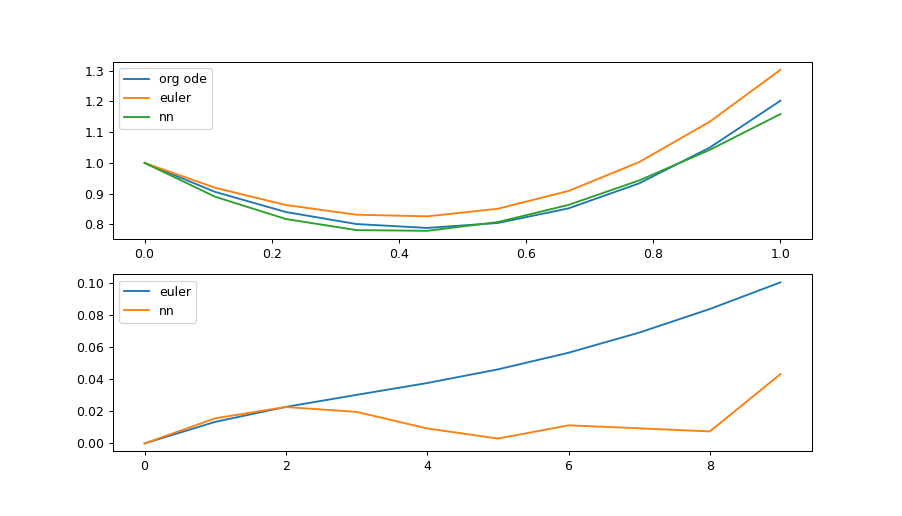
\includegraphics[width=0.8\textwidth]{./pic/ans.png}
        \caption{真实解-Euler解-NN解}\label{fig:ANS}
    \end{figure}

\end{frame}


%----------------------------------------------------------------------


\section{总结与展望}

\begin{frame}{结论}
    \begin{exampleblock}{优势}
		\begin{enumerate}
			\item 无需在意差分格式的构造
			\item 可以达到极高的精度
			\item 理论上随着神经元和隐含层的增多,损失函数的值趋于$0$
			\item 训练一个模型,可以解一类方程\cite{DBLP}
		\end{enumerate}
	\end{exampleblock}
	
	\begin{alertblock}{劣势}
		\begin{enumerate}
			\item 针对简单的微分方程仍需多次迭代,此时收敛速度无法与差分方法相提并论
			\item 重点在于试解的构造
			\item 不仅要求神经网络的导数,还要求试解的导数,这会导致第一点
			\item 编程更为复杂
		\end{enumerate}
	\end{alertblock}
\end{frame}
%----------------------------------------------------------------------
\begin{frame}{展望}
    \begin{block}{神经网络在PDE上的应用}
		\begin{enumerate}
			\item 分子蛋白运动模拟(上一次中科院研究员卢本卓老师201讲座,未找到参考文献)
			\item 求解薛定谔方程\cite{solve_mxde, SolvingXDE}
			\item 神经网络不仅在数学工程,而且在生物分子、物理化学都在发挥着更重要的作用
		\end{enumerate}
	\end{block}
\end{frame}

%----------------------------------------------------------------------

\begin{frame}{Home Page}

\begin{enumerate}
	\item \url{https://t-xiaomeng.github.io/}
	\item \url{https://github.com/T-XiaoMeng}
	\item \url{https://github.com/T-XiaoMeng/nn_for_pde}
\end{enumerate}

\end{frame}
%----------------------------------------------------------------------
\begin{frame}{致谢}
\begin{center}
	{\Huge\calligra Thanks!}
\end{center}
\end{frame}


%----------------------------------------------------------------------
\begin{frame}[allowframebreaks]
    \frametitle{参考文献}
    \printbibliography
	%\bibliographystyle{plain}
	%\bibliography{nkthesis}
\end{frame}

\end{document}
